%%%%%%%%%%%%%%%%%%%%%%%%%%%%%%%%%%%%%%%%%%%%%%%%%%%%%%%
%%                  Thermomechanical                 %%
%%%%%%%%%%%%%%%%%%%%%%%%%%%%%%%%%%%%%%%%%%%%%%%%%%%%%%%
\chapter{Thermomechanical models for product remanufacturing of a turbine rear structure}
\chaptermark{Thermomechanical models for product remanufacturing of a turbine rear structure}
\label{ch:thermomechanical}
%%%%%%%%%%%%%%%%%%%%%%%%%%%%%%%%%%%%%%%%%%%%%%%%%%%%%%%

In this chapter, we introduce the industrial application example used to demonstrate our methodologies in Chapters \ref{ch:scalableSBD}, \ref{ch:TSEcont}, and \ref{ch:stohasticopt}. We define the thermomechanical model used to analyze the deposition process used to remanufacture the product. The product considered in this thesis is the \ac{TRS}. The models developed in this section are specific to the deposition of various stiffener geometries on the \acf{TRS}. However, the simplifications to the thermomechanical analysis used to compute the residual effects of directed energy deposition on the substrate are generalizable to any deposit and substrate.

A \ac{TRS} is a structural aeroengine component at the turbine exhaust. It must sustain thermal and structural loads during flight due to exhaust gases while mounting the engine to the wing structure. Analysis of the component in the industry involves multiple disciplines (aerodynamic, structural, and thermal). 

We consider the deposition of a stiffener on the \ac{TRS} to support higher loading requirements. The first step of the analysis involves a thermomechanical model to compute the residual stresses in the structure ($\sigma_{v1}$). 

Any subsequent loading of the \ac{TRS} during operation results in a new stress state ($\sigma_{v2}$). The mean and amplitude of the initial and final stress states are used to compute the safety factor against low-cycle fatigue as a structural performance metric. We consider two different load cases in Chapters \ref{ch:scalableSBD} and \ref{ch:TSEcont}. However, the calculation of the safety factor against low-cycle fatigue is independent of the load case used in the analysis.

The following section outlines the thermomechanical models used to predict the residual stresses that result from the \ac{AM} deposition process. {\color{red} All the loadcases presented in this thesis take advantage of the cyclic symmetry of the \ac{TRS} by restricting the analysis to one sector.}

%========================== THERMOMECHANICAL ===========================%
\section{Thermomechanical modeling}
\label{sec:thermomech}

The \ac{DED} of the stiffener increases the thickness of the outer casing as shown in Figure~\ref{fig:TRSoverview}. 

\begin{figure}[h!]
	\centering
	\subfloat[TRS schematic \label{fig:TRSiso}]{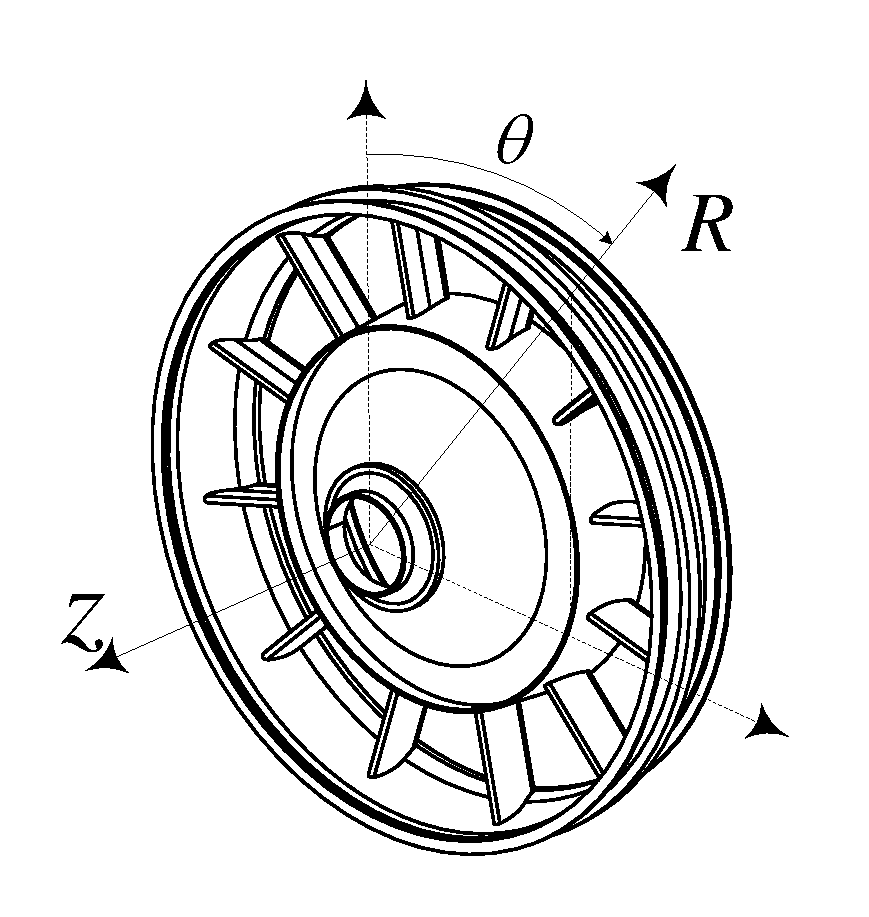
\includegraphics[width=0.3\textwidth]{1a_TRS_isometric}} \hspace{0.1\textwidth}%
	\subfloat[Deposition variables \label{fig:stiffdims}]{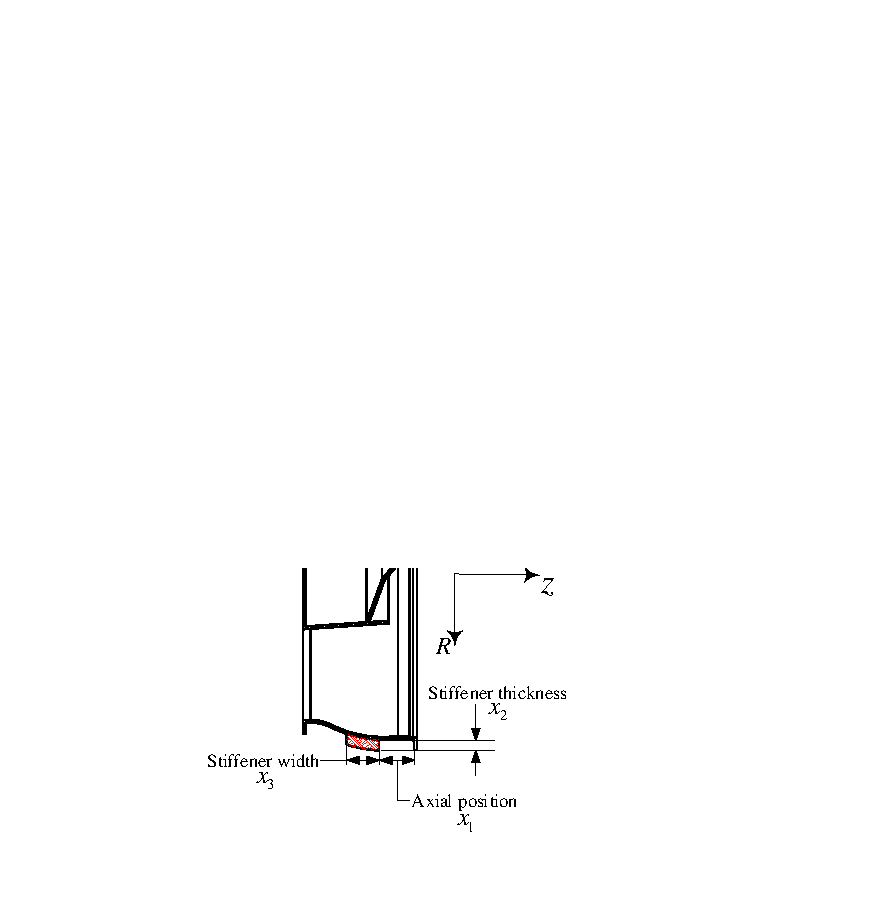
\includegraphics[width=0.4\textwidth]{1b_TRS_overview}}	
	\caption{TRS stiffener example}
	\label{fig:TRSoverview}
\end{figure}

Comprehensive thermomechanical models feature a coupled transient heat transfer and fluid flow model to accurately calculate the transient temperature field. The temperature field is used for residual stress and distortion modeling \cite{Mukherjee2017}. Complex physical processes govern the temperature field making its computation intensive. Computations of the temperature field involve various simplifications and assumptions to make the calculations tractable. \citeauthor{Manvatkar2011} consider a \ac{FEA} conduction model for calculating the transient temperature field due to a moving Gaussian heat source on the substrate \cite{Manvatkar2011}. The problem of a moving heat source on an infinite plate was formulated and solved analytically by \citeauthor{rosenthal1946theory} \cite{rosenthal1946theory}. The Rosenthal model is used for cases where there is limited heat conduction in the through thickness dimension typical of thin plates \cite{Goldak1984}. The \ac{TRS} outer casing where the stiffener is to be deposited has a through thickness dimension considerably smaller than its width and circumference allowing us to approximate the heat source by a Gaussian heat source as in the Rosenthal model.

The melt pool dimensions are estimated from the transient thermal model to determine the deposit width and depth. Figure~\ref{fig:gaussian} shows the details of the thermomechanical simulations for determining deposit size. A Gaussian heat source scanning the surface of a substrate at a constant speed ${V}$ has a heat flux distribution given by
%
\begin{equation}
	Q(r,\theta,t) = \dfrac{P_{\textrm{laser}}}{\pi{r_l}^2 D_p}e^{-2\left(\frac{r-{V}t}{r_l}\right)^2}, \label{eg:gaussian}
\end{equation}
%
where ${r_l}$ is the laser beam radius, $P_{\textrm{laser}}$ is the laser power, and $D_p$ is the depth of penetration of the laser source \cite{rosenthal1946theory}. The coordinates $r$ and $\theta$ are defined on the surface of the deposit as shown in Figure~\ref{fig:gaussianheat}. 

\begin{figure}[h!]
	\centering
	\subfloat[Gaussian heat source\label{fig:gaussianheat}]{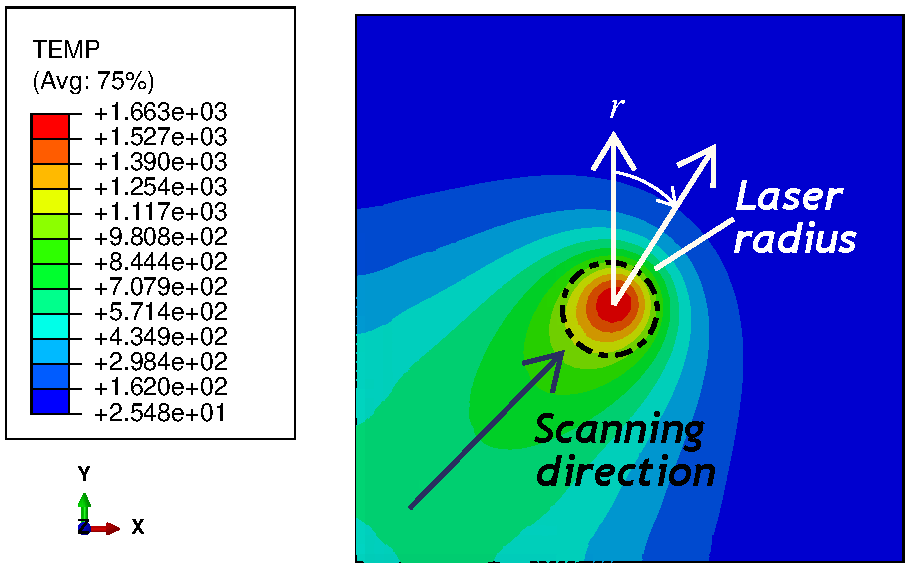
\includegraphics[width=0.45\textwidth]{2a_guassian_heat}} \hspace{0.1\textwidth}%
	\subfloat[Melt pool  \label{fig:pooldims}]{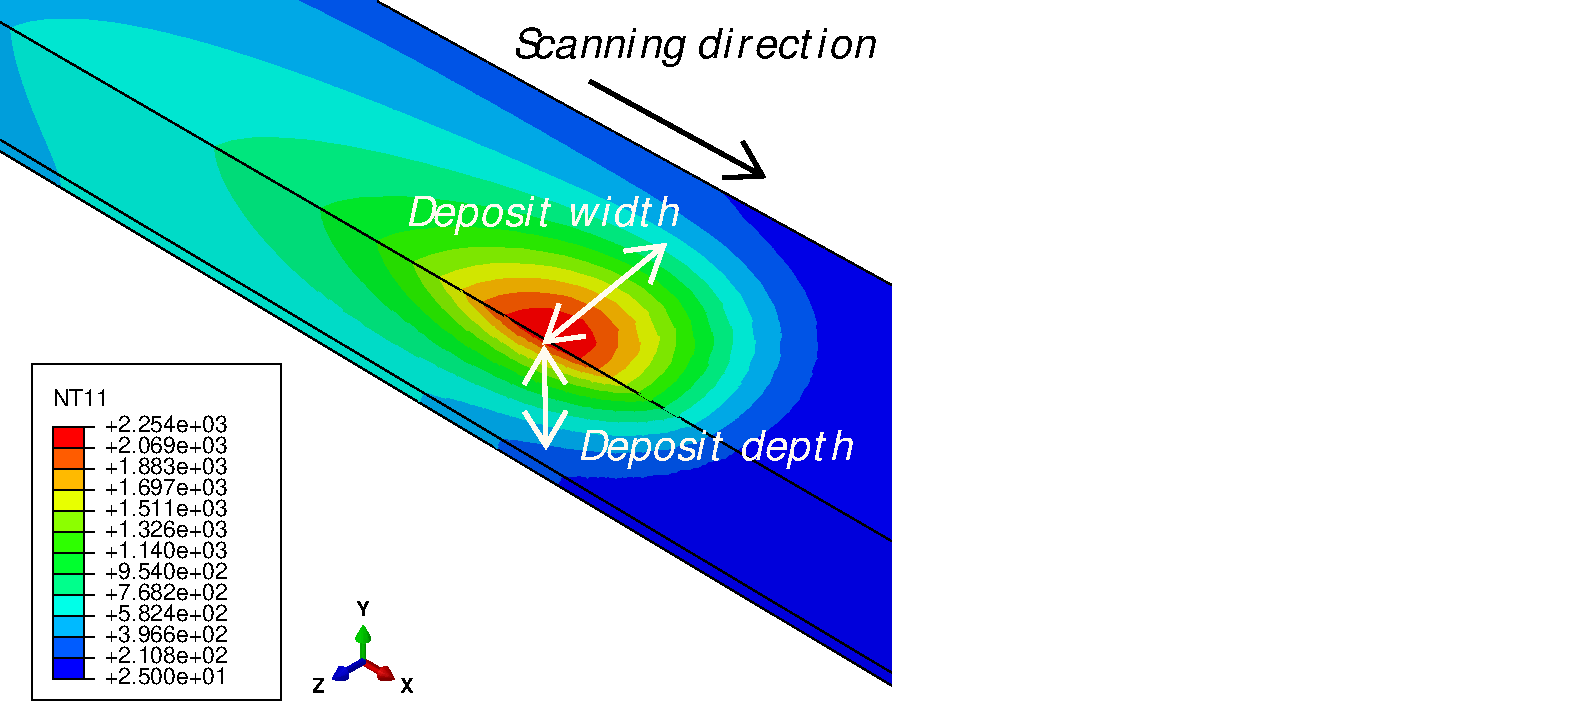
\includegraphics[width=0.29\textwidth]{2b_pool_dims}}	
	\caption{Heat conduction for a moving Gaussian heat source}
	\label{fig:gaussian}
\end{figure}

The resulting deposit width $D_w$ and depth $D_d$ are used to partition the stiffener geometry into $n_l$ by $n_d$ deposits in the axial and radial directions, respectively, where $n_l = \round{x_3/D_w}$ and $n_d = \round{x_2/D_d}$. 

For deposition on the \ac{TRS} outercasing, a further simplification of the transient conduction model can be made by applying the heat flux uniformly on the surface of the deposit \cite{Nickel2001}. We use a static model with a uniformly distributed heat flux to compute residual stresses. This idealization (relative to using a transient heat transfer model) reduces the number of variables and parameters involved and alleviates computational cost by exploiting TRS symmetry without sacrificing accuracy excessively.

Each deposit is heated uniformly by an equivalent heat flux that supplies the same energy as a moving Gaussian heat source scanning the entire deposit surface. The power at $t=0$ is given by the surface integral of the heat flux over an infinite plane
%
\begin{equation}
	\label{eq:power}
	P(t=0) = \dfrac{P_{\textrm{laser}}}{\pi{r_l}^2 D_p} \Int_{0}^{2\pi} \Int_{0}^{\infty} e^{-2\left(\frac{r}{r_l}\right)^2} \,rdr\,d\theta = \dfrac{P_{\textrm{laser}}}{\pi{r_l}^2 D_p}\dfrac{\pi{r_l}^2}{2} = \dfrac{P_{\textrm{laser}}}{2D_p}.
\end{equation}
%
The power per unit depth $P(t=0)$ is multiplied by the scanning time $t_{scan}$ to obtain the heat energy input to the deposit. The scanning time is calculated for each stiffener by dividing total distance traveled by the heat source (stiffener length) by the scanning speed $t_{scan} = L/V$. $A_{\textrm{stiff}}$ is the surface area of the stiffener where heat is applied. These values are obtained from the geometry of the stiffener using \ac{CAD} tools.

The energy is divided by an equivalent step time $t_{\textrm{step}}$ used for static thermal analysis in lieu of a transient thermal analysis to obtain the equivalent uniformly distributed power per unit depth $P_{\textrm{eqv}}$. $P_{\textrm{eqv}}$ is divided by the area of the deposit $A_{\textrm{stiff}}$ to yield the equivalent heat flux per unit depth
%
\begin{equation}
	\label{eq:powereqv}
	Q_{\textrm{eqv}} = \dfrac{P_{\textrm{laser}}}{2D_{p}}\dfrac{t_{\textrm{scan}}}{t_{\textrm{step}}}\dfrac{1}{A_{\textrm{stiff}}}.
\end{equation}

A special case of stiffener is the circumferential stiffener shown in Figure~\ref{fig:TRSoverview}. For this type of stiffener, Equation~(\ref{eq:powereqv}) can be simplified by setting $L = 2\pi R_{\textrm{outer}}$, where $R_{\textrm{outer}} = 0.5$ m is the radius of the outer casing of the \ac{TRS}. This results in $t_{scan} = 2\pi R_{\textrm{outer}}/V$. The deposit surface area becomes $A_{\textrm{deposit}} = 2\pi {R_{\textrm{outer}}}D_w$ to yield the equivalent heat flux per unit depth
%
\begin{equation}
	\label{eq:powereqvcirc}
	Q_{\textrm{eqv}} = P(t=0)\dfrac{2\pi R_{\textrm{outer}}}{V}\dfrac{1}{t_{\textrm{step}}}\dfrac{1}{2\pi {R_{\textrm{outer}}}D_w} = P(t=0)\dfrac{1}{{V}t_{\textrm{step}}D_w} = \dfrac{P_{\textrm{laser}}}{{2V}t_{\textrm{step}}D_wD_p}.
\end{equation}
%
Here, we assume that the radius of the deposit is equal to the radius of the outer casing $R_{\textrm{outer}}$ since the thickness of the deposit is small relative to the outer casing.

An example of the application of $Q_{\textrm{eqv}}$ to the surface of a circumferential deposit layer is shown in Figure~\ref{fig:depload}.

\begin{figure}[h!]
    \centering
    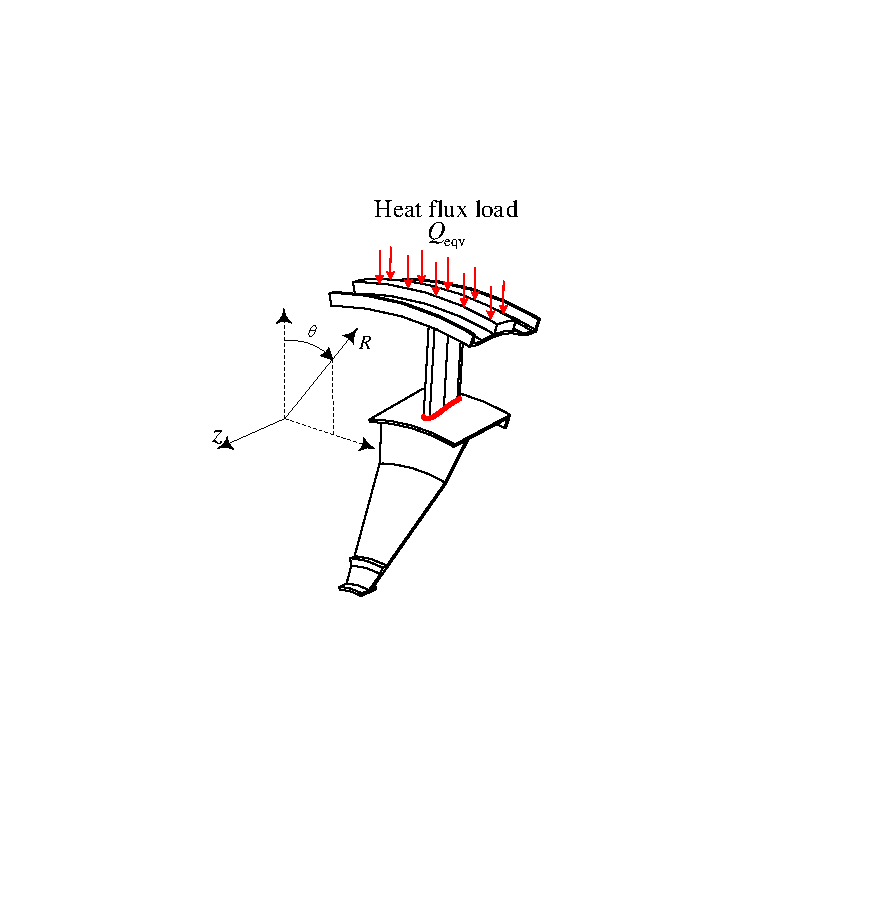
\includegraphics[width=0.4\textwidth]{3a_heat_load.pdf}
    \caption{ \label{fig:depload} Deposition load }
\end{figure}

After obtaining the thermal gradients due to the application of the heat flux load, the corresponding thermal stresses are computed. The stresses that persist after removal of the heat flux load are the residual stresses. These residual stresses are inherent in the structure and affect the structural performance of the \ac{TRS} during subsequent operational loads. 

The maximum and minimum residual principal stresses along the circumference of the \ac{TRS} outer casing are shown in Figure~\ref{fig:Sprinciple} for both static and transient models. Table~\ref{table:validation} summarizes the utilized parameter values for this comparative study.

\begin{table}[h!]
\centering
\renewcommand{\arraystretch}{1.0}% Wider
\small\addtolength{\tabcolsep}{-5pt}
\caption{Comparison of transient and static models: parameter values}
\label{table:validation}
\begin{tabular}{lcccc}
\hline\hline
\bf Parameter & \bf Notation & \bf Units & \bf Value \\\\ \hline
Stiffener axial position & $x_1$ & mm & 80.0  \\
Stiffener thickness  & $x_2$ & mm & 4.0  \\
Stiffener width & $x_3$ & mm & 23.5  \\
Laser Power & $P_{\textrm{laser}}$ & W & 3,889.13 \\ 
Laser beam radius & ${r_l}$ & mm & 13.63 \\ 
Scanning speed& ${V}$ & mm/s & 5.0 \\ 
Number of layers & $n_l$ & - & 2\\
Number of deposits (transverse) & $n_d$ & - & 1\\
Deposit depth  & $D_d$ & mm & 2.01\\
Deposit width  & $D_w$ & mm & 25.0 \\
Deposit surface area  & $A_\textrm{deposit}$ & mm$^2$ & \num{8.304e4} \\
Equivalent heat flux per unit depth & $Q_\textrm{eqv}$ & W/mm$^3$ & 0.8138 \\
\hline\hline
\end{tabular}
\end{table}

In all our analyses throughout the thesis, the scanning speed is considered constant at a nominal value of $V = 5$ mm/s.

\begin{figure}[h!]
	\centering
	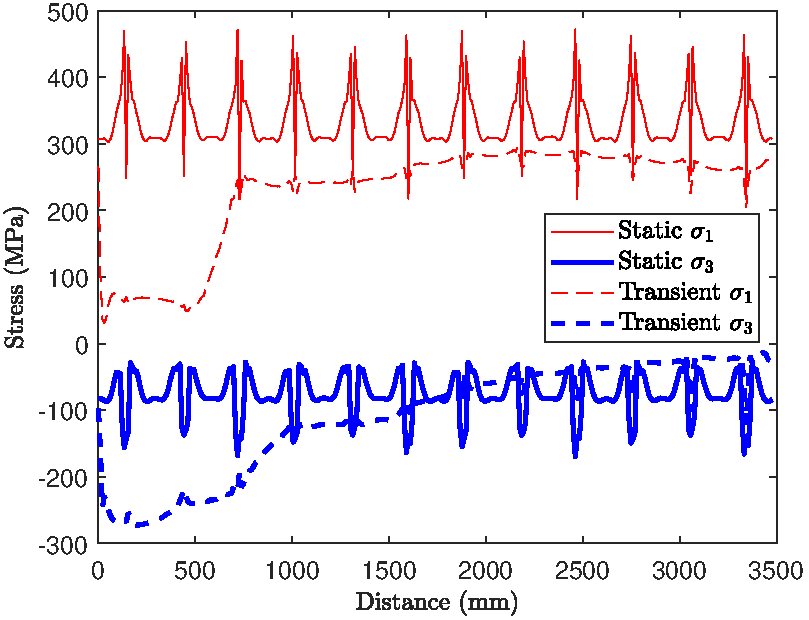
\includegraphics[width=0.6\textwidth]{6_residual_stresses.pdf}
	\caption{ \label{fig:Sprinciple} Spatial distribution of principle residual stresses along the circumference of the \ac{TRS} obtained using transient and static models}
\end{figure}

The principal stresses provide an indication of the compressive or tensile nature of the stress state and will be used in subsequent failure analysis to determine the safety factor. There is a general agreement in the value of the predicted stresses with lower values recorded for the transient model due to the time taken by the substrate to reach steady state temperatures as the heat source scans its surface. Furthermore, the static model overpredicts the maximum principal stress making it a more conservative choice for thermomechanical modelling.

In the following section we describe the different load cases that the \ac{TRS} may experience in operation.

%============================= LOAD CASES ==============================%
\section{Load cases applied to turbine rear structure}
\label{sec:loadcases}

The \ac{TRS} experiences a number of thermal and mechanical loads due to the exhaust gases it directs while providing structural support to the engine. Two significant load cases are used for the analyses in this thesis to address the effect of changing parameters on the functionality of the \ac{TRS}.

We describe the first load case in the following section.

%---------------------------------------------------------------------%
% Pressure load case
\subsection{Pressure load case} \label{subsec:iploadcase}

\begin{figure}[h!]
    \centering
    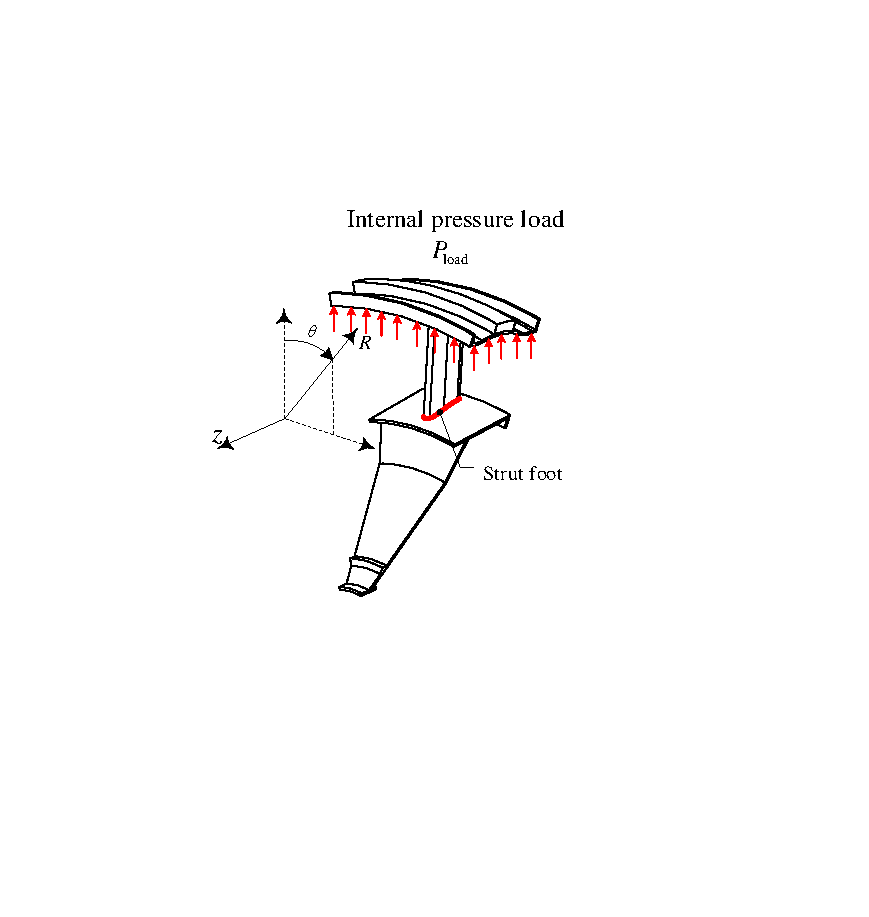
\includegraphics[width=0.4\textwidth]{3b_pressure_load.pdf}
    \caption{ \label{fig:ipload} \ac{TRS} pressure load case }
\end{figure}

The first load case is due to the internal pressure $P_{\textrm{load}}$ applied on the outer casing of the \ac{TRS} by the hot exhaust gases. A pressurization/depressurization cycle on a sector of the \ac{TRS} is shown in Figure~\ref{fig:ipload}. The load case is cycled and is used to compute the expected fatigue life of the \ac{TRS} using low-cycle fatigue calculations. The stress state at the foot of a strut (shown in Figure~\ref{fig:ipload}) is monitored before and after the load case to obtain the initial and final Von Mises stresses $\sigma_{v1}$ and $\sigma_{v2}$, respectively. Note that $\sigma_{v1} \neq 0$ due to the residual stress state in the structure from prior thermomechanical loads. 

We now describe the thermal loadcase due to the temperature of the exhaust gases.

%---------------------------------------------------------------------%
% Thermal load case
\subsection{Thermal load case} \label{subsec:thermalloadcase}

The \ac{TRS} shown in Figure~\ref{fig:TRSiso} is subject to thermal loads due to temperature gradients experienced during operation. The temperature profile of a \ac{TRS} during operation is shown in Figure~\ref{fig:thermalloads}. These temperature loads are specified by the \ac{OEM} engine architect to the \ac{TRS} component supplier in the form of changing parameters.

\begin{figure}[h!]
	\centering
	\subfloat[Safety factor calculation domain \label{fig:TRSisothermal}]{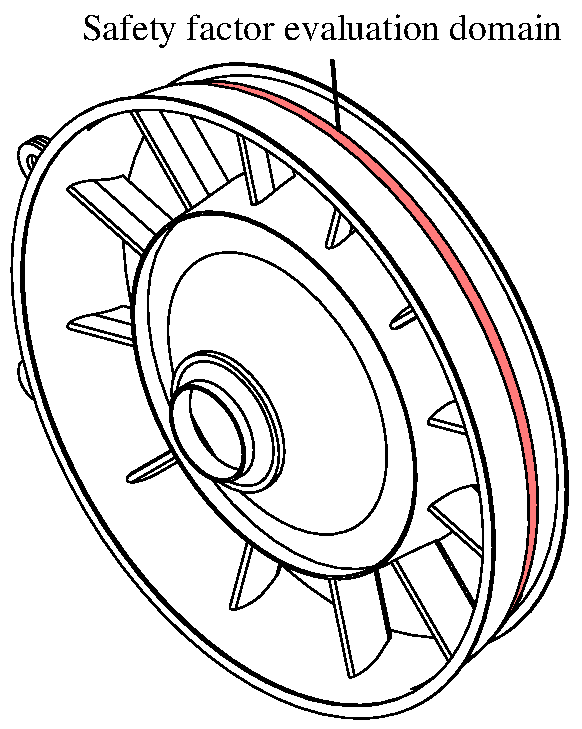
\includegraphics[width=0.275\textwidth]{5a_TRS_isometric}} \hspace{0.1\textwidth}%
	\subfloat[Thermal loads \label{fig:thermalloads}]{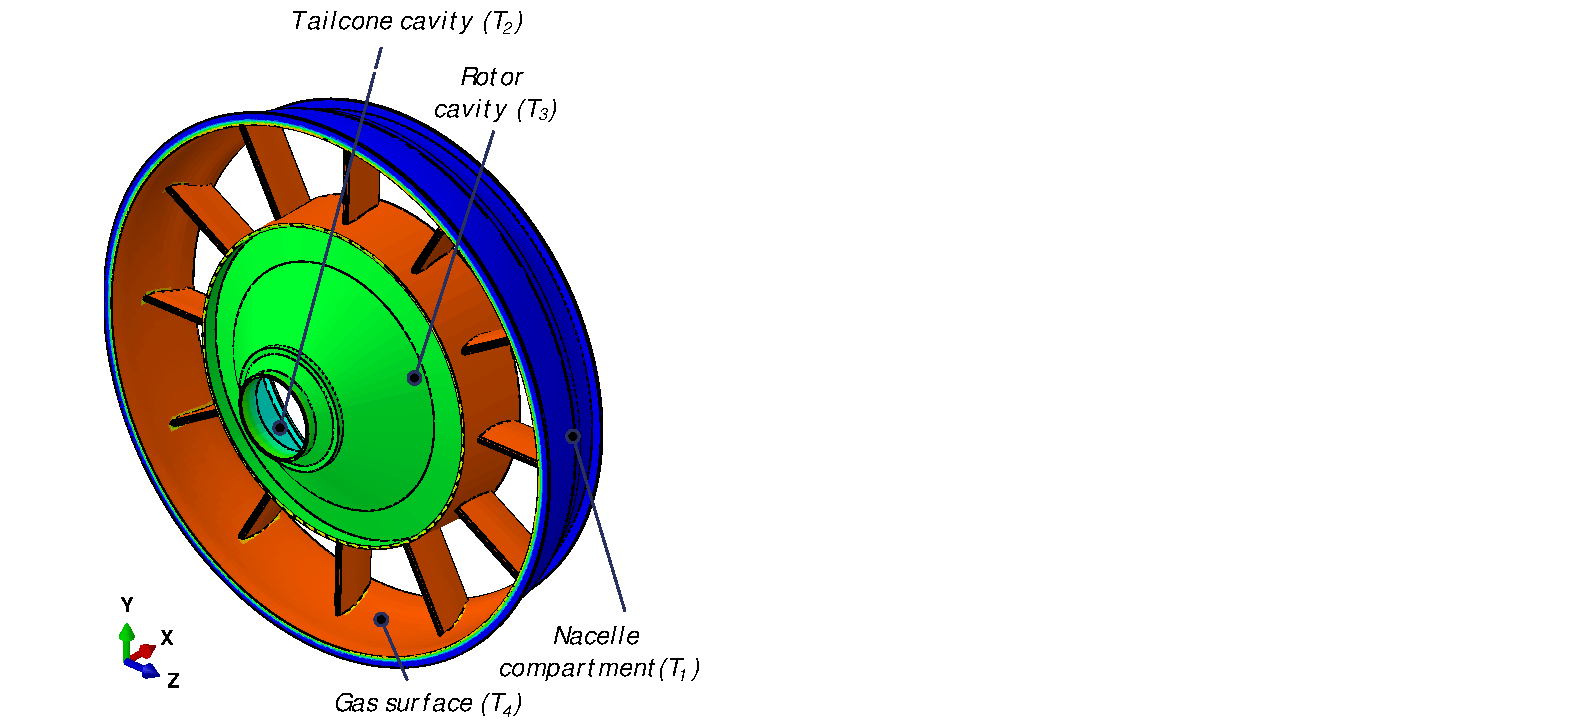
\includegraphics[width=0.3125\textwidth]{5b_thermal_loadcase}}
	\caption{\ac{TRS} thermal load case}
	\label{fig:thermalloadcases}
\end{figure}

The thermal load case is cycled and is used to compute the expected fatigue life of the \ac{TRS} using low-cycle fatigue calculations. The stress state at the midsection of the outer casing is recorded before and after the load case to obtain the initial and final Von Mises stresses $\sigma_{v1}$ and $\sigma_{v2}$, respectively.

The structural analyses presented for the thermomechanical, pressure, and thermal load cases are performed using a \ac{FE} simulation model which is computationally expensive. As a result, we will construct surrogates for these models in Chapters \ref{ch:scalableSBD}, \ref{ch:TSEcont}, and \ref{ch:stohasticopt} to alleviate the computational effort involved in exploring the design and parameter spaces for these application examples.

We explain how the safety factor $n_{\textrm{safety}}$ is computed for these load cases in the following section.

%---------------------------------------------------------------------%
% Fatigue calculation
\subsection{Low-cycle fatigue analysis} \label{subsec:fatigueanalysis}

We use the initial and final Von Mises stresses $\sigma_{v1}$ and $\sigma_{v2}$ obtained before and after the application of either load case described earlier to compute the safety factor against low-cycle fatigue.

The midrange stress ($\sigma_m = -\textrm{sign}(\sigma_P)\left( \sigma_{v1} + \sigma_{v2}\right) / 2$) and the amplitude stress ($\sigma_a = \left| \sigma_{v1} - \sigma_{v2}\right| / 2$) are calculated, where $\textrm{sign}(\sigma_P)$ is the sign of the pressure given by the sum of the principle stresses ($\sigma_P = -(1/3) (\sigma_1 + \sigma_2 + \sigma_3)$) and provides of measure of the compressive or tensile state of the stress. A negative $\sigma_P$ implies tension while a positive value implies compression. The failure locus is determined by the modified Goodman criterion for low-cycle fatigue as shown in Figure~\ref{fig:GMcrit}. The endurance limit ($S_e$), yield stress ($\sigma_y$), and ultimate strength ($S_{ut}$) are defined as parameters and are obtained from mechanical design handbooks \cite{Budynas2015}. The number of lifecycles to failure is estimated from W{\"o}hler's relation ($N_f = \left(\sigma_{\textrm{rev}}/a\right)^b$), where $a$ and $b$ are empirical constants. The safety factor is calculated as $n_{\textrm{safety}} = 1/\left({\frac{\sigma_a}{S_e}+\frac{\sigma_m}{S_{ut}}}\right)$ for each load case. 

\begin{figure}[h!]
    \centering
    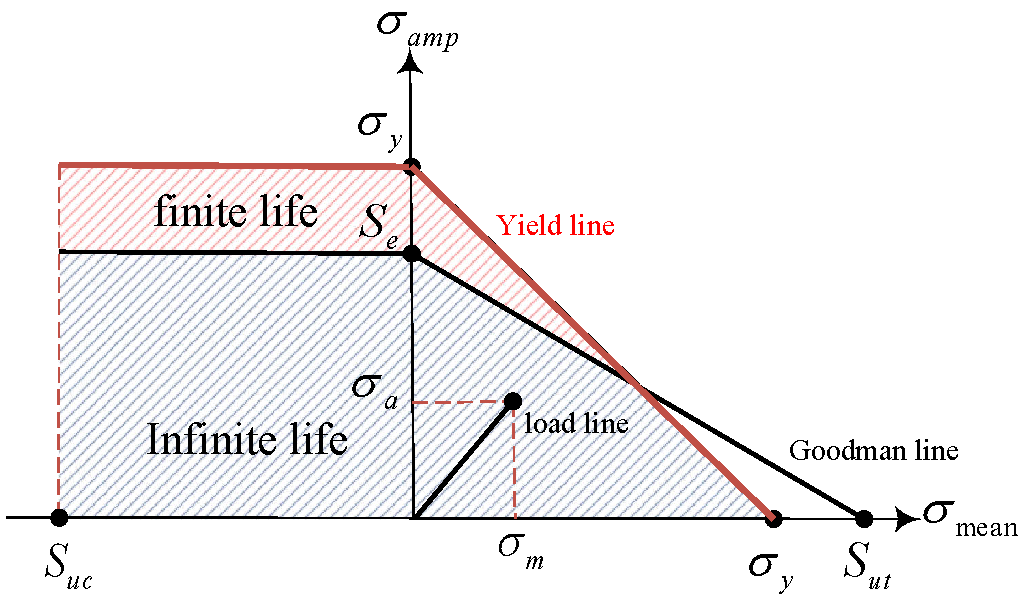
\includegraphics[width=0.7\textwidth]{4_Fatigue_loading.pdf}
    \caption{ \label{fig:GMcrit} Modified Goodman criterion }
\end{figure}

The safety factor $n_{\textrm{safety}}$ is used as a structural performance metric throughout this thesis. We now summarize all the relevant model inputs and outputs for the thermomechanical models and loadcases.

%============================== SUMMARY ================================%
\section{Summary}
\label{sec:thermosummary}

This chapter presented the industrial application example that will be used throughout the thesis to demonstrate the developed frameworks. The chapter defined the thermomechanical model and two loadcases that the \ac{TRS} experiences in operation. The loadcase parameters and outputs are summarized in Tables \ref{table:modelinputs} and \ref{table:modeloutputs} respectively. Some parameters in Table \ref{table:modelinputs} can change and are denoted by ranges. They will be elaborated on during the analyses in the following chapters.

\begin{table}[h!]
	\centering
	\renewcommand{\arraystretch}{1.0}% Wider
	\normalsize\addtolength{\tabcolsep}{-5pt}
	\caption{Relevant model inputs}
	\label{table:modelinputs}
	\begin{tabular}{lcc>{\centering\arraybackslash}p{3cm}>{\centering\arraybackslash}p{2cm}}
	\hline\hline
	\bf Parameter & \bf Notation & \bf Units & \bf Value \\ \hline
	Stiffener axial position & $x_1$ & mm & $91 \pm 54$ \\
	Stiffener thickness  & $x_2$ & mm & $6 \pm 4$ \\
	Stiffener width & $x_3$ & mm & $25 \pm 15$  \\
	Laser Power & ${P_{\textrm{laser}}}$ & W & $3750 \pm 250$\\ \hline
	Internal pressure load  & ${P}_{\textrm{load}}$ & MPa & $2 \pm 0.5$ \\ 
	Deposit melting point & $T_m$ & $^o$C & $1,500 \pm 100$ \\
	Substrate base width & $W_{\textrm{total}}$ & mm & $137.5 \pm 17.5$ \\
	Nacelle temperature & $T_1$ & $^{o}$C & $300 \pm 100$ \\ 
	Tailcone temperature & $T_2$ & $^{o}$C & $400 \pm 100$ \\ 
	Rotor temperature & $T_3$ & $^{o}$C & $450 \pm 100$ \\ 
	Gas surface temperature & $T_4$ & $^{o}$C & $600 \pm 100$ \\
	\hline
	%================================================================
	Laser beam radius & ${r_l}$ & mm & 14.2 \\ 
	Scanning speed& ${V}$ & mm/s & 5.0 \\ 
	Laser penetration depth & $D_p$ & mm & 5.0 \\
	%================================================================
	\hline\hline
	\end{tabular}
\end{table}

\begin{table}[h!]
	\centering
	\renewcommand{\arraystretch}{1.0}% Wider
	\normalsize\addtolength{\tabcolsep}{-5pt}
	\caption{Relevant model outputs}
	\label{table:modeloutputs}
	\begin{tabular}{lcc}
	\hline\hline
	\bf Output    & \bf Notation & \bf Units \\ \hline
	Number of layers & $n_l$ & - \\
	Number of deposits (transverse) & $n_d$ & - \\
	Deposit depth  & $D_d$ & mm \\
	Deposit length  & $D_l$ & mm \\
	Deposit width  & $D_w$ & mm \\
	Deposit surface area  & $A_\textrm{stiff}$ & mm$^2$ \\
	Deposit length  & $L$ & mm \\
	Scanning time  & $t_\textrm{scan}$ & s \\
	Equivalent heat flux  & $Q_\textrm{eqv}$ & W/mm$^2$ \\
	Safety factor against low-cycle fatigue & $n_{\textrm{safety}}$ & - \\
	Number of lifecycles to failure (${P}_{\textrm{load}}$)& $N_f$ & - \\
	Deposition temperature & $T_\textrm{deposit}$ & $^o$C \\
	\hline\hline
	\end{tabular}
\end{table}

We describe the methodology for obtaining scalable design solutions for product remanfuacturing in the following chapter. The internal pressure loadcase described in Section~\ref{subsec:iploadcase} will be used to demonstrate this framework. The thermal loadcase described in Section \ref{subsec:thermalloadcase} will be used for demonstrating the design margin allocation tool developed in Chapter \ref{ch:TSEcont}.